\documentclass[12pt]{extarticle}\usepackage[utf8]{inputenc}\usepackage{cite}\usepackage{graphicx}\title{An Empirical Discussion on Golden Ratio, $\Phi$}\author{Nesar Ul Alam}\date{July 2019}

\begin{document}\maketitleGolden Ratio, first depicted and described by Euclid in the golden age of Greek Knowledge, discusses about a fundamental characteristics in the number theory. A number is said to be in a Golden Ratio if their ratio is found to be same as the ratio of their sum to the larger of the two. The greek letter $\phi$ is used as the symbol of Golden Ratio. The value of $\phi$ is 1.61803398875. The number itself is irrational. The term ``Golden" has been used as it is considered to be aesthetically pleasing and examples of the ratio can be drawn from the nature itself.In terms of mathematics, the Golden Ratio can be described in many different ways. However, for the sake of simplicity, we must start from the first description of the ratio, as depicted by Euclid, the line segment theory. It goes in this way- 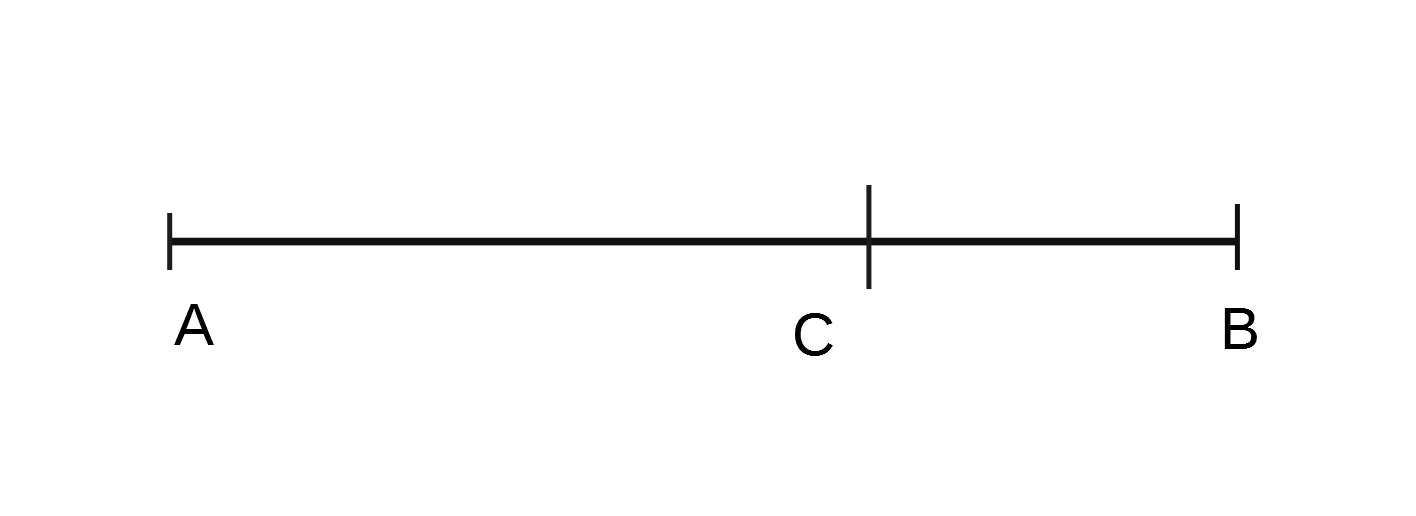
\includegraphics[]{ffUntitled.png}As can be seen from the image, length of $AB$ is greater than that of $AC$ and $AC$ is greater than $CB$. if $AC$ $:$ $CB$ is equals to $AB$ $:$ $AC$, then we can conclude that the line has been cut in a Golden Ratio \cite{livio2008golden}. \bibliographystyle{plain}\bibliography{M335}\end{document}

